\chapter{Redesign of A Long HCDR3 Antibody}
\label{chap:chapter4}
\section{Introduction}
Recent studies described the isolation of a number of human monoclonal antibodies (mAbs) with broad and potent neutralizing activity, many of which exhibit unusual features \citep{Bonsignori:2011dq,McLellan:2011dg,Walker:2009cd,Walker:2011ew}. As discussed in the chapter \ref{chap:chapter1}, broadly neutralizing antibodies to HIV generally contain high levels of somatic mutations or exceptionally long HCDR3 lengths. The V2/V3 neutralizing class of anti-HIV antibodies which includes PG9, PG16, CH01, CH04, PGT141 and PGT145 all have a long heavy chain complementarity determining region 3 (HCDR3) and possess unique structural elements that interact with complex protein and glycan features reaching past a large bulk of complex and high mannose glycans to interact with a short segment termed strand-C5. These antibodies share similar neutralization sensitivity including glycan knockouts and strand-C point mutations that interact with interface residues \citep{DoriaRose:2012if,Doores:2010gn}.  For PG9 and its clonally related sibling PG16, crystal structures have been solved in complex with V1/V2 gp120 showing that these antibodies both engage the epitope with their HCDR3 loop in a similar ways with the exception of glycan interactions \citep{Pancera:2013ev}. While PG16 prefers hybrid type glycans at position N173 (HIV variant HXBc2 numbering), PG9 has little dependence.

\subsection{Experimental Rationale}
As an extension of my work in chapter \ref{chap:chapter3} that considers antibodies with exceptionally long HCDR3s, I chose to pursue a redesign study of the broadly neutralizing antibody PG9. This allowed me to ask relatively simple questions that may have broad and far-reaching implications for antibody and vaccine design. Is the native sequence of PG9 optimal for binding and neutralization potency? PG9 and PG16 converge on structure and binding modes but they are encoded by different sequences. Therefore, I hypothesized that the HCDR3 loop of PG9 could be redesigned to achieve improved affinity of binding, increased potency, and breadth of neutralization for diverse HIV strains.

There has already been precedent for chimeric antibodies of PG9/PG16 where a motif from PG16 responsible for the recognition of complex type glycans was transposed onto PG9 in order to increase potency and breadth. This approach allowed PG9, which initially had no preference for complex type glycans at position 173 (HIV variant HxBC2), to bind those glycan types with stronger affinity, while retaining PG9s ability to bind high mannose type antibodies. This chimeric antibody extended the breadth of PG9 with a small subset of mutations on the light chain CDR3 loop termed PG9-RSH \citep{Pancera:2013ev}.

In addition, NIH45-46, a broadly neutralizing mAb that shows structural mimicry for CD4 and closely resembles VRC01, was mutated by one amino acid in the HCDR2 loop \citep{Scheid:2011js,Diskin:2011hl}. The mutation was not designed computationally; rather, the investigators aligned the bound structure of NIH45-46 with CD4 and observed that CD4 had a hydrophobic burial of a phenylalanine residue at position 54 (figure \ref{fig:figure4_1} A). This interaction was recapitulated in another antibody, VRC03, with a tryptophan residue at position 54. The wild-type amino acid G54 did not fully recapitulate the CD4 interaction as it left a large gap between the gp120 outer domain and the HCDR2 (figure \ref{fig:figure4_1} A). The investigators predicted that a mutation to either a hydrophobic residue, such as the phenylalanine of CD4, or the tryptophan used by VRC03 would increase potency by increasing the mimicry of CD4. Indeed, a mutation to tryptophan at position 54 (NIH45-46\textsubscript{G54W}) increased neutralization potency for a majority of the viral strains tested and up to 2,000-fold for one of the strains (figure \ref{fig:figure4_1} B,C).

Using the high-throughput sequencing data obtained in chapter \ref{chap:chapter3}, I predicted I could map the energy landscape of the HCDR3 structure using the \rosetta~scoring function. That is, we sought to look at amino acid sequences at all positions of the HCDR3 and determine their overall level of fitness for each position. Does PG9 contain the optimal sequence for the HCDR3 loop? If I didn't see a complete recovery of PG9 sequence, I could then predict that other sequence combinations or point mutations exists that enhance fitness of the HCDR3 and may increase breadth and potency to HIV. Again, these mutations would then be carried over to the laboratory to be tested experimentally with binding and neutralization assays.

\begin{figure}
   \centering
   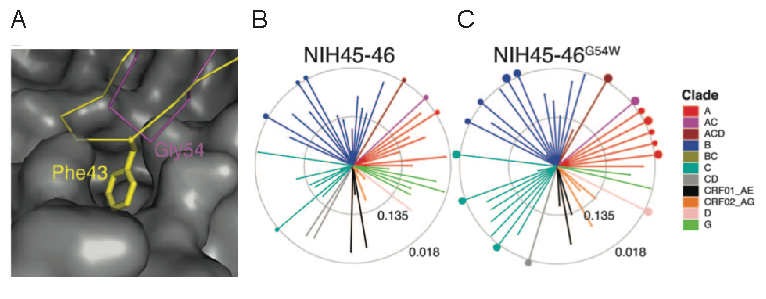
\includegraphics{images/chapter4/figure4_1.pdf} % requires the graphicx package
   \caption[Rational Design of NIH45-46 to Increase Neutralization Potency]{Rational design of NIH45-46 to increase neutralization potency. The gp120 bridging sheet is shown as a surface representation with CD4 shown in yellow and NIH45-46 shown in purple (A). Spider plots showing the neutralization profile for NIH45-46 and point mutant NIH45-46G54W are shown. The length of the line corresponds inversely with the \ic~value. Each circle represents a ten-fold change in \ic~(B,C). Figure adapted from \citep{Diskin:2011hl}}
   \label{fig:figure4_1}
\end{figure}

\section{Mapping the Energy Landscape of PG9}
\label{sec:mapping}
I retrieved the atomic resolution structure of the complex of mAb PG9 with the CAP45.2.00.G3 variant V1/V2 scaffold from the Protein Data Bank (PDB ID:3U4E) \citep{McLellan:2011dg}. A large number of naturally-occurring 30-amino-acid (30 AA) length HCDR3 antibody sequences was identified in antibody gene repertoires from high-throughput sequencing of antibody amplicons from RNA of B-cells of HIV-negative donors. Retrieval of this dataset is discussed at great length in chapter \ref{chap:chapter3}. A heat map of amino acid occurrences is displayed in figure \ref{fig:figure4_2} A for 30-length HCDR3s. Diversity among the repertoires is seen for all positions 98-118. The sequence conservation at the 5' and 3' ends of the HCDR3 sequences, 96-98 and 118-125, respectively, are due to the ARD motif that make up the 5' end of a canonical neck of a long HCDR3 loop or the J\textsubscript{H}6 template sequence, which was seen in a majority of long HCDR3 sequences \citep{North:2011dv,Briney:2012ib}. Between these two stretches of sequence conservation, I observed large sequence diversity. Glycine, tyrosine and serine are generally tolerated at all positions, while proline, lysine and methionine are found less frequently between positions 99-117 (figure \ref{fig:figure4_2}A). This phenomenon is well established in loop unstructured regions connecting beta-sheets in antibodies \citep{Minuchehr:2005wc,De:2005in}.  This propensity for a structure to tolerate a diverse set of amino acid sequences was the focus of the current study. The idea is that there is tremendous sequence space to be explored in 30-length HCDR3s that may further enhance breadth and specificity.

My methods are described fully in the appendix \ref{sec:appendixIII}, but use the same general protocol as described in Chapter \ref{chap:chapter3}. I used the software suite \rosetta~to determine the ability of diverse 30-AA HCDR3 sequences to tolerate the structure of the hammerhead configuration of the HCDR3 of PG9 by threading 4,000 naturally-occurring unique sequences over the PG9 HCDR3 structure. Once the sequences are threaded, I scored them by evaluating the \rosetta~scoring function for each position. The contribution to the total score of each position (the sum of all scoring terms of \rosetta), which can be thought of as thermal stability, and the contribution to the binding energy (the total score in complex subtracted from the total score in a separated interface) of each position were evaluated. These scores are best viewed as heat maps (figure \ref{fig:figure4_2} B,C). These two metrics, total score and binding energy, can be summed to determine what I define as the mutational ``fitness''. In this way, I trimmed the tremendous sequence space as viewed in the heat map in figure \ref{fig:figure4_2} A, to a focused sequence space containing mutations that advantageously affect either thermal stability or binding energy. These metrics are shown in the heat maps of figure \ref{fig:figure4_2} A-B, offer an advantage structure-based metrics in exploring design. As expected, PG9 itself scored as the most fit sequence for a majority of amino acid positions for the HCDR3 (dots plotted in figure \ref{fig:figure4_2}).

\begin{figure}
   \centering
   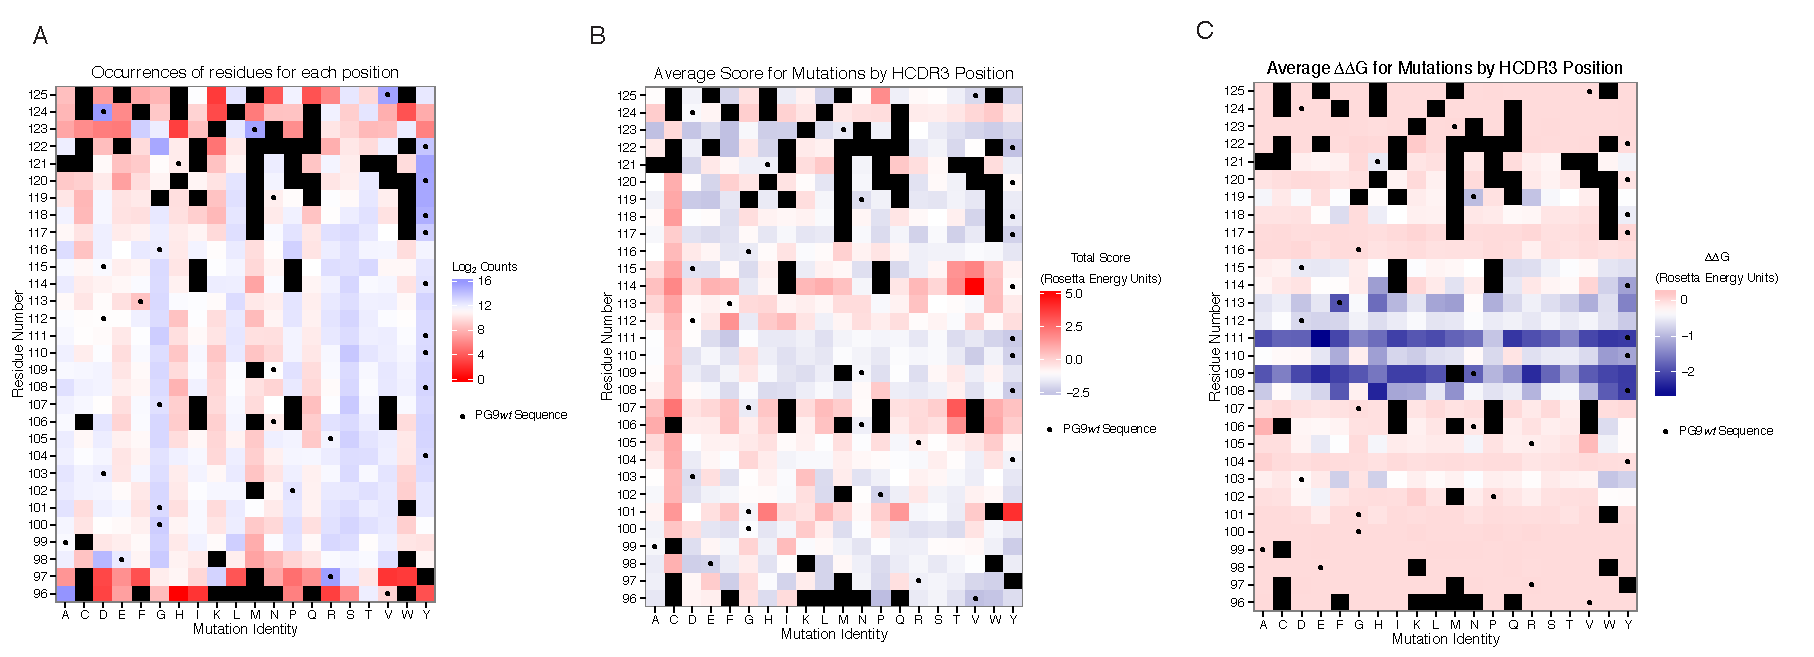
\includegraphics[width=.99\textwidth]{images/chapter4/figure4_2.pdf} % requires the graphicx package
   \caption[Amino Acid Usage and Energy Landscape of PG9]{Amino acid usage and energy landscape of PG9. Mutation identity is plotted on the x-axis with each of the positions in the 30-length HCDR3 on the y-axis. The usage of each amino acid is shown in a log\textsubscript{2} blue-red scale counted from 26,422 HCDR3 sequences (A). 4,000 randomly selected sequences were chosen and their individual score from the \rosetta~energy function is shown on a blue-white scale (B). The contribution of the same 4,000 randomly selected sequences contribution to binding energy is shown on a blue-white scale (C). For A-C, the PG9 native sequence is shown as a dot.
}
   \label{fig:figure4_2}
\end{figure}

\section{Redesign of PG9}
Rather than pick the amino acids that had the best fitness for each position, I allowed a complete redesign of the PG9 HCDR3 loop using \rosettadesign. My reasons for choosing this method rather than a simple matrix lookup generated in the previous section were two fold:
\begin{enumerate}
\item Complete redesign can account for cooperative mutations. Consider position 99 that has a wild-type alanine for PG9. My heat maps for the energy landscape predicted that there are many more favorable mutations I could make including an aspartic acid, asparagine or tyrosine. However, I are unaware if the new mutations have the potential to be cooperative. That is, do the aspartic acid, asparagine, or tyrosine require neighboring mutations to be fully stable? The complete redesign allowed me to account for cooperative mutations while recapitulating the energy landscape predicted in section \ref{sec:mapping}.
\item Using a combination of filters and movers based on my specific design goals, I prevented \rosetta~from designing amino acids too far away from the original PG9 sequence, position, and structure. I can also tell the \rosetta~scoring function to optimize for binding energy, thermal stability, or a combination thereof. This information would be lost on a matrix lookup \citep{Fleishman:2011ji,Kaufmann:2010ea,Kuhlman:2000tc}.
\end{enumerate}

Again, the full design protocol is detailed in the in the Appendix (Chapter \ref{sec:appendixIII}) and follows the same basic structure as the redesign of sequences detailed in Chapter \ref{chap:chapter3}. I designed 1,000 decoys allowing small docking perturbations and minimal backbone movement. I filtered the design to optimize for binding energy. That is, only obtain sequences if they were better than binding energy of PG9\textit{wt}.

The easiest way to view the sequences returned from the PG9 redesign is with a sequence logo representation (figure \ref{fig:figure4_3} A). The x-axis is the PG9\textit{wt} sequence while the height of the letters at each position, measured in bit, measure \rosetta's preference for that amino acid given the nature of the design challenge. As expected from the observations from the energy landscape (figure 4.2), the original PG9 sequence was returned for a majority of the positions, considering the evolutionary sequence bias of the PG9 structure (nature optimizes sequences for the PG9 structure).  Regardless, anytime an amino acid was returned in 10\% or more of the models, I further inspected the design fitness of the mutation.

I measured the design fitness as a sum of the difference in total energy from wild-type sequence and the difference in binding energy from the wild-type sequence ($\Delta\Delta$G + total score). For some of the positions, multiple amino acids were suggested by \rosetta~rather than the wild-type amino acid sequence (figure \ref{fig:figure4_3} A,B). For most positions, the design fitness was negligible, falling above the noise threshold (figure \ref{fig:figure4_3} B, dashed-line). However design at antibody amino acid positions 104, 109, 115, 120, and 123 (PDB numbering) suggested alternative amino acids that were predicted to benefit HCDR3 fitness for the antibody-V1/V2 interaction (figure \ref{fig:figure4_3} B).

I wanted to make sure that each of these mutations made intuitive sense upon examination of the structure. I viewed each mutation in context and compared it to the wild-type amino acid. My aim was to determine if this mutation was an artifact and to confirm that it was non-cooperative with other mutations, that is, the mutation enhances fitness alone and not in cooperation with many other mutations made to the sequence. This is because I wanted to retain as much of the PG9\textit{wt} sequence as possible. These visual inspections are shown in figure \ref{fig:figure4_3} B in the table, with a full justification given. If a mutation was found to be non-cooperative, and still enhanced fitness, it was considered for experimental characterization (green squares), N109Y and D115N met these criteria. I also considered N109L and a cooperative mutation A99S and Y120N as they showed strong stabilization through inter-HCDR3 loop hydrogen bonding. I also made one combinatorial mutation that included the double cooperative mutant A99S-Y120N and two single mutations D115N and N109L. This variant is simply referred to as PG9\_4MUT (figure \ref{fig:figure4_3}C). I did not pursue further evaluation of designs that appeared to compromise the structural integrity of the HCDR3 loop by visual inspection.

\begin{figure}[!t]
   \centering
   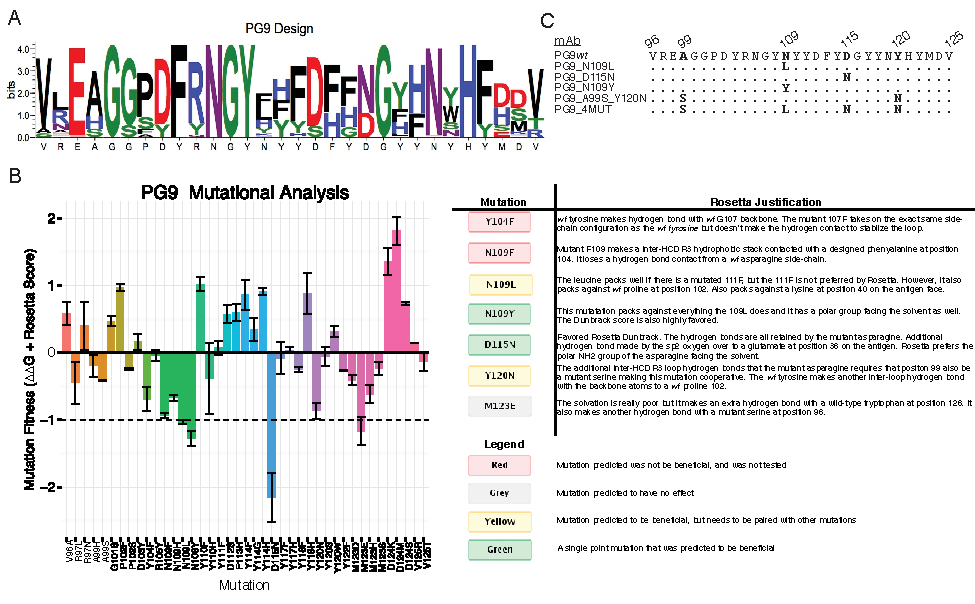
\includegraphics[scale=1.5,width=.99\textwidth]{images/chapter4/figure4_3.pdf} % requires the graphicx package
   \caption[Redesign of PG9 HCDR3]{Redesign of PG9 HCDR3. For 1,000 designed models, the sequences returned are best viewed as a sequence logo. The x-axis is the PG9\textit{wt} sequence while the y-axis represents the preference, measured in bit, of the amino acid identities, identified by the height of the letter (A). For sequences that were returned greater than 10\% of the time, I manually inspected their fitness as a measure of binding energy and thermal stability (y-axis). Some positions had more than one amino acid favored and are grouped by color. \rosetta~noise is plotted as a dashed line at -1 REU. The more negative a mutation is, the more it is beneficial to the PG9 complex. Each mutation is visually inspected and justified (table). They are either a single point mutations that benefits, a cooperative mutation that benefits, no change in fitness, and detriment to fitness, as green, yellow, grey, and red, respectively (B). The final mutations that are chosen to be carried out experimentally are three point mutations and two combinations thereof (C).}
   \label{fig:figure4_3}
\end{figure}


\section{Experimental Characterization of PG9 Variants}
For the five mutational variants of PG9, I used a similar cloning strategy as described in Chapter \ref{chap:chapter3} that takes advantage of unique cloning sites between the HCDR3 5' and 3' ends. Each of the variants expressed well, and protein concentration was not a limiting factor. I began by testing all the variants against a 15 antigen mix of gp120 Env proteins to qualitatively measure binding. In this preliminary study, the double mutant, A98S-Y120N produced a significantly lower signal than that of PG9, and this variant was not considered further.

PG9\textit{wt} does bind to some gp120 monomers (although PG9\textit{wt} also can neutralize HIV variants for which it does not bind to monomer). I used a panel of representative gp120 monomers from HIV clades B and C to perform screening for binding of PG9 variants to Env \citep{Li:2006kv,Li:2005go}. The results were in good agreement with previous studies of the binding of PG9\textit{wt} to gp120 monomers \citep{McLellan:2011dg}. For these PG9 variants, I calculated half-maximal effective concentration (\ec) values. For each gp120 monomer tested, the PG9 variants N109L and N109Y exhibited 2.3-14.2 fold stronger binding than did PG9\textit{wt} (figure \ref{fig:figure4_4}), while PG9 variant D115N exhibited comparable binding energies to PG9\textit{wt}. PG9\_4MUT exhibited 2-100 fold reduced binding. This finding is most likely due to the A98S-Y120N mutation that I had previously determined as deleterious.

I also determined the \ec for binding of these PG9 variants to a recombinant form of native gp140 trimer that is recognized by PG9, termed BG505-SOSIP.66419-21. In these assays, both PG9 variants N109L and N109Y exhibited 3.5- or 5.9-fold stronger binding respectively than PG9\textit{wt}. In addition to the stronger binding affinity, the variant N109Y bound to trimer with a complete sinusoidal curve and a strong maximum signal mimicking the binding profile of the glycan-specific mAb 2G12, which is optimal for binding to the trimer \citep{Sanders:2013gm}  (figure \ref{fig:figure4_4}A). The extreme change in maximal signal is intriguing, and may suggest changes in valency of P9 to the trimer although this has not been confirmed \citep{Julien:2013jp}.

I next tested the panel of redesigned PG9 variants and PG9\textit{wt} for neutralizing activity against a panel of viruses displaying PG9-susceptible or -resistant HIV Env molecules, using a TZM-bl neutralization assay \citep{Montefiori:2009hj}. The PG9 variant N109Y exhibited increased neutralization potency for all viruses tested, including viral variants for which PG9\textit{wt} did not have activity (i.e., had neutralization concentration >33 \mcml) (figure \ref{fig:figure4_4}B). Remarkably, PG9 variant N109Y neutralized at 3.72 \mcml~an HIV strain with the N160A mutation that removes the glycan at that position that is required for binding of PG9\textit{wt}6. The PG9 variant N109L also exhibited an increase in potency against HIV strains compared to PG9\textit{wt}, although not at the same level as the PG9 variant N109Y. In all assays tested, N109Y and N109L consistently had enhanced breadth and potency.

The magnitude of the improvement to neutralization was modest in some cases, but the improvement was consistent over a wide variety of HIV strains and showed significant p-values (p < 0.05) for 10 out of the 15 virues for PG9\_N109Y and 4 out of the 15 viruses for N109L (table \ref{tab:table4_1}). Using a meta-analysis for all p-values tested gave a p-value of 5.44 x 10\textsuperscript{-15} and 7.36 x 10\textsuperscript{-4} indicating a strong statistical significance observed for the increase in potency of neutralization for PG9\_N109Y and PG9\_N109L respectively. I also found a decrease in potency to be statistically significant for 8 out of the 15 viruses tested for PG9\_D115N and a combined p-value of 2.64 x 10\textsuperscript{-8}.


\begin{figure}[!t]
   \centering
   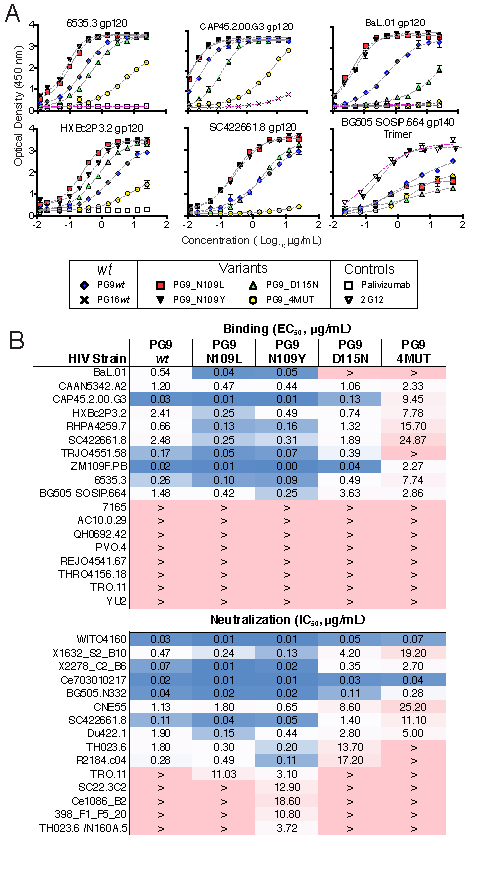
\includegraphics{images/chapter4/figure4_4.pdf} % requires the graphicx package
   \caption[Experimental Analysis of PG9 Variants]{Representative binding curves are shown with the optical density at 450 nm shown on the y-axis plotted against the log\textsubscript{10} concentration in \mcml~on the x-axis (A). All \ec values were calculated from the curves like the ones shown in (A) as well as the neutralization \ic~against a 15 virus panel (B)}
   \label{fig:figure4_4}
\end{figure}

\begin{table}[!t]
    \centering
    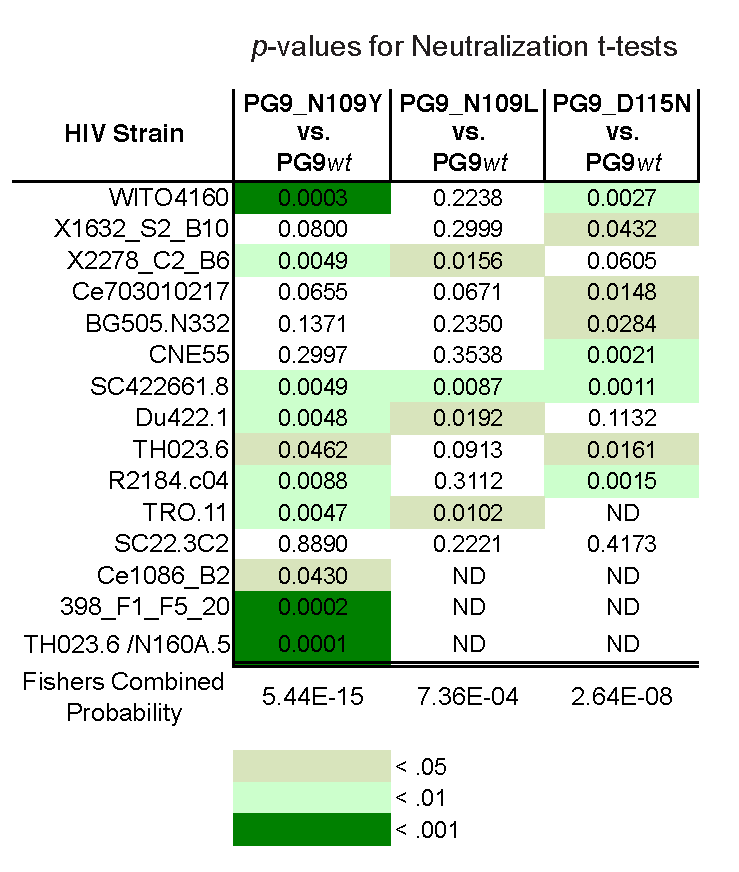
\includegraphics[scale=.8]{tables/chapter4/table4_1.pdf}
    \caption[Statistical Tests for Neutralization Breadth of PG9 Variants]{Statistical tests for neutralization breadth of PG9 variants. The \ic~values between each neutralization assay for PG9\_N109Y, PG9\_N109L, and PG9\_D115N were compared with a student's non-parametric t-test against the \ic~value for PG9. They are shown as p-values for each viral variant. A total p-value for each antibody is shown as a Fisher's combined probability.}
    \label{tab:table4_1}
\end{table}


\section{Models to Corroborate Experimental Outcome}
I sought to develop a predictive model to determine the molecular basis for the increased potency and breadth of these PG9 variants using the \rosetta~scoring function. I generated three different mutants D115N, N109L and N109Y, which were compared to that of PG9\textit{wt} using the \rosetta~scoring function (figure \ref{fig:figure4_5} A). I analyzed the top 25 models for each of the scoring metrics shown. my scoring metrics were binding contribution for the HCDR3, binding for the full complex, total score for the bound and unbound structure ($\Delta\Delta$G). For each metric calculated, I observed statistically significant improvements in HCDR3 stabilization for N109L or N109Y (p < 0.01 or p < 0.001, respectively), but none of my other metrics.

Upon examination of the predicted structures of the top scoring models, I found the antibody position 109 was located on an antiparallel beta-sheet at the apical tip of the HCDR3 forming a hydrophobic pocket near the interface of the antigen and apical tip (figure \ref{fig:figure4_5} B). The pocket is formed by antibody residues Y104, Y110 and P102 of the antibody heavy chain (PDB numbering). In addition, D167 on the antigen face makes contact with this position. Examination of the structure revealed that the bulk of the hydrophobic amino acid at this position of the pocket contributes to stabilization of the preferred structure of HCDR3. The small hydrophobic bulk of the asparagine fills the pocket, but as the bulk increased to a leucine and then a tyrosine, the predictive model suggested a further stabilization of the HCDR3 loop. In addition, the polar group on the end of the designed tyrosine at position 109 points into solvent space, recapitulating the effect of the polar head of the original asparagine PG9\textit{wt}t.

It is important to note that since I calculate the stabilization as the total energy of the HCDR3 loop, it can be dissected into the individual scoring terms given by \rosetta. These are both described in the chapters \ref{chap:chapter1} and the appendix \ref{chap:appendix}. I have broken the total score down for the HCDR3 loop in figure \ref{fig:figure4_6}. There is little deviation for most of the scoring terms, however, both the attractive force term, the solvation term in the \rosetta~scoring function are improved for the N109L and N109Y mutations. In addition the N109Y shows a favored $\pi$-$\pi$ term. These interactions are accounted for in the model as the N109 position is between a large hydrophobic bulk. In addition, position N109Y also achieves a more favorable $\pi$-$\pi$ stacking interaction with residue Y110 compared to PG9\textit{wt} as the aromatic ring of the designed tyrosine can stack with position 110.

\begin{figure}[!t]
   \centering
   \includegraphics[width=.99\textwidth]{images/chapter4/figure4_5.pdf} % requires the graphicx package
   \caption[Predictive Models of PG9 Variants that Enhanced Binding]{The top 25 models for each binding metric are analyzed. The x-axis is each of the variants and the y-axis is the \rosetta~energy units. The metrics are decomposed by binding energy (A) and thermal stabilization (B). Just the HCDR3 is considered (left) or the entire complex (right). Surface representation of position 109. Green is the antigen labeled V1/V2, blue is the HCDR3 loop, dark green is the N160 glycan. Each mutation of interest is shown as a sphere representation that is adjusted to fit the \rosetta~ atom radius. Spheres are colored by atom type with oxygen in red, nitrogen blue, and carbon in grey. Hydrogens are removed for clarity.}
   \label{fig:figure4_5}
\end{figure}


\begin{figure}[!t]
   \centering
   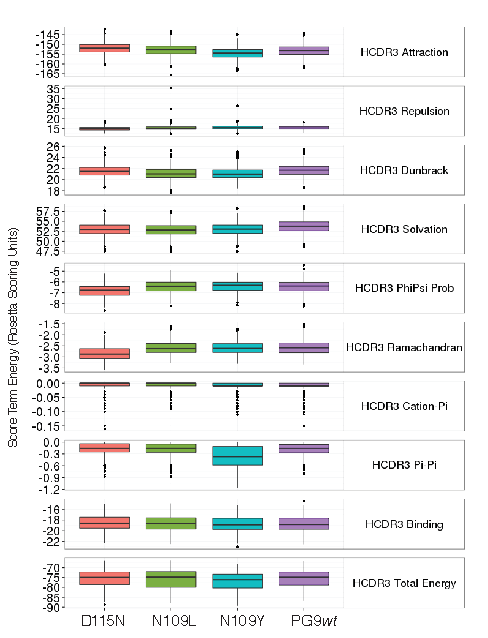
\includegraphics[scale=1.4]{images/chapter4/figure4_6.pdf} % requires the graphicx package
   \caption[Decomposed Scoring Terms for PG9 Variants]{Decomposed scoring terms for PG9 variants. The contribution of individual scoring terms to the total energy score for the HCDR3 loop for each mutation. The predictive model used 1000 simulations for each variant. Each scoring term for \rosetta is shown in the y-axis panel. The y-axis value is the score for that energy term.}
   \label{fig:figure4_6}
\end{figure}


\section{Discussion}
These results have important implications for antibody and vaccine design. The studies reveal the power of \rosetta~computational modeling to design antibodies with improved function using structural predictions. Remarkably, the improvements in neutralizing potency and breadth observed here for PG9 variants were achieved not by altering interface residues, but rather by increased stability of HCDR3 loops discovered using a holistic model to determine stability of an antigen-antibody complex. This finding is consistent with recent mutagenesis experiments showing that non-contact residues are essential for antigen recognition by many broadly neutralizing antibodies to HIV \citep{Klein:2013iz}. Non-contact residues in antibody frameworks contribute to high affinity binding by facilitating formation and stability of a pre-configured, low energy binding site \citep{Willis:2013dd,Manivel:2000wk,Marlow:2010jl,Wedemayer:1997wn,Schmidt:2013ka}. Optimally configured binding sites form ordered paratopes that pay a smaller entropic penalty upon forming antibody-antigen complexes \citep{Marlow:2010jl}.

This work shows the efficiency of combining \rosettadesign~computational experiments with expert knowledge and wet laboratory validation experiments. For a HCDR3 loop of 30-AAlength, 600 single point mutants are possible, and the number of variants with more than one mutation is enormous. From this large potential set of mutated antibodies, \rosettadesign~identified a focused panel of candidate PG9 variants, from which a small subset was considered favorable, and two of five experimentally tested variants exhibited enhanced potency and breadth of neutralization. The computational experiments provided tremendous enrichment for variants with improved binding, but as expected was not completely accurate. For example, although the model suggested that D115N would have the greatest increase in fitness (figure 4.3) this variant was not improved in activity.
The negative result is important, as \rosetta~often predicts design failures, and their exploration is fundamental in improving the \rosetta~algorithm and scoring function for the most accurate representations of experimental observation. This computational-experimental feedback has been instrumental to my work and will be the target of my future directions.

With the combination of high-throughput sequencing, rapid threading, and experimental feedback, I complete a robust bioinformatics pipeline that can rapidly test antibodies for improvement based solely on their \silico~predictions. The results here suggest that there probably is a diversity of antibodies with long and structured HCDR3s that fit the PG9 topology in nature with HIV neutralizing activity that have yet-to-be discovered. I hypothesize this conclusion from three parts of evidence:
\begin{enumerate}
\item Examination of the energy landscape of PG9 suggests that there are mutations that are predicted to be better suited for the PG9 topology.
\item PG9 and PG16 diverge in sequence but converge on a structural topology and have approximately identical specificities and potencies \citep{McLellan:2011dg,Pejchal:2010fp,Pancera:2010hh}.
\item I have discovered point mutations in PG9 that enhance breadth and specificity.
\end{enumerate}
These yet to be discovered antibodies may possess higher HIV inhibitory activity and breadth than the antibodies that are currently in hand. Additional antibody exploration efforts may be worthwhile to identify antibodies of interest with which to design epitope mimetic vaccines, as has been successfully recently implemented \citep{Correia:2014jp,Jardine:2013hb}.



\section{Conclusions and Future Directions}
Two observations may be critical to explore in this current work. The maximum signal difference in the binding assay for the BG505-SOSIP trimer between my variants and the PG9\textit{wt} is worth further exploration. Julien and colleagues observed that PG9 recognizes the trimer asymmetrically \citep{Julien:2013jp}. There are three epitopes displayed on the apical tip of the gp120 trimer, yet PG9 only has a 1:3 valency of binding to HIV Env. The molecular mechanism for this trimeric preference is unavailable due to the high resolution of the structure reported in the study, but the model suggests that PG9 may interact with the adjacent N160 glycan. Could the mutation cause a change in valency in binding? This change would explain to the maximal signal change in my binding assay. Future experiments could replicate the study performed by Julien \textit{et al.} either with high-resolution gel-filtration or isothermal titration calorimetry.

Another observation is the glycan independence of the binding of the N109Y variant. It was originally thought that the binding of any V1/V2 binding antibody would depend on glycans at position N160 and N156/N1706 considering they not only block the recessed C-strand epitope, but make considerable binding contributions for both PG16 and PG9 \citep{McLellan:2011dg,Pancera:2013ev}. It was demonstrated that these glycans are needed for recognition and specificity, as mutational experiments completely abrogated neutralization. I was able to replicate that finding, however, my variants still neutralized HIV glycan knockout viruses, albeit, at much lower potency (3.52 \mcml). It is worth replicating this ``glycan independence'' with many more viral species that have been mutagenized to knockout glycans. I have already begun to pursue this aim.

Finally, I can attempt to repeat the application of this entire technology to mutagenesis of PG9's sibling, PG16. I already have the mutational candidates, and the antibody cDNAs are being synthesized at the time of this writing. It is important to keep in mind that PG16 specific to the trimeric-Env, so variants can only be tested with neutralization experiments or if I synthesize stable trimer \citep{Sanders:2013gm}.




